\documentclass[12pt]{article}
\usepackage{graphicx}
\usepackage{float}
\begin{document}
\title{Statistics 12, Lab 3}
\date{February 19th, 2019}
\author{Michael Wu\\UID: 404751542}
\maketitle

\section*{Exercise 1}

\paragraph{a)}

I ran the following code.
\begin{verbatim}
linear_model <- lm(soil$lead ~ soil$zinc)
summary(linear_model)
\end{verbatim}
This output the following statistics.
\begin{verbatim}
Call:
lm(formula = soil$lead ~ soil$zinc)

Residuals:
    Min      1Q  Median      3Q     Max
-79.853 -12.945  -1.646  15.339 104.200

Coefficients:
             Estimate Std. Error t value Pr(>|t|)
(Intercept) 17.367688   4.344268   3.998 9.92e-05 ***
soil$zinc    0.289523   0.007296  39.681  < 2e-16 ***
---
Signif. codes:  0 ‘***’ 0.001 ‘**’ 0.01 ‘*’ 0.05 ‘.’ 0.1 ‘ ’ 1

Residual standard error: 33.24 on 153 degrees of freedom
Multiple R-squared:  0.9114,	Adjusted R-squared:  0.9109
F-statistic:  1575 on 1 and 153 DF,  p-value: < 2.2e-16
\end{verbatim}

\paragraph{b)}

I ran the following code.
\scriptsize
\begin{verbatim}
plot(soil$lead ~ soil$zinc, xlab="Zinc Concentration (ppm)",
     ylab="Lead Concentration (ppm)", main="Lead vs. Zinc in Soil")
abline(linear_model, col="red", lwd=2)
\end{verbatim}
\normalsize
This generated the following plot.
\begin{figure}[H]
    \begin{center}
        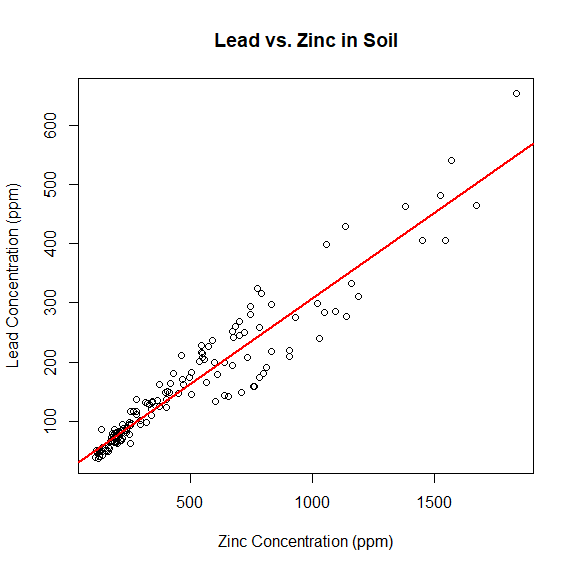
\includegraphics[width=4.5in]{exercise1b.png}
    \end{center}
\end{figure}

\paragraph{c)}

I ran the following code
\scriptsize
\begin{verbatim}
plot(linear_model$residuals ~ soil$zinc, xlab="Zinc Concentration (ppm)",
     ylab="Lead Residuals (ppm)", main = "Lead vs. Zinc in Soil Residuals plot")
abline(a=0, b=0, col="red", lwd=2)
\end{verbatim}
\normalsize
This generated the following plot.
\begin{figure}[H]
    \begin{center}
        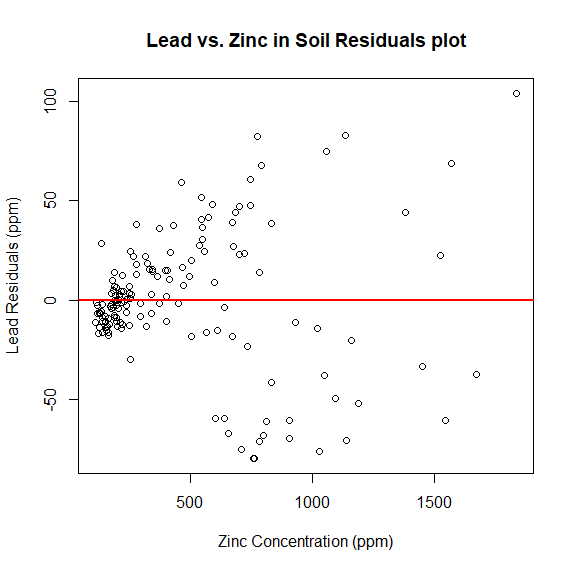
\includegraphics[width=4.5in]{exercise1c.png}
    \end{center}
\end{figure}

\paragraph{d)}

The equation of the regression line is the following.
\[y=0.289523x+17.367688\]

\paragraph{e)}

We would expect the lead concentration to be 306.89 ppm.

\paragraph{f)}

We would expect the lead concentration to be 28.95 ppm higher.

\paragraph{g)}

The R-squared value is 0.9114. In this context it means that 91.14\% of
the variation in the lead concentration can be determined by the variation in zinc
concentration.

\paragraph{h)}

I believe that linearity, symmetry, and are met for this data. The data appears
very straight and the residuals look symmetrical. However,
the condition for equal variance is not met. The residuals appear to become
more spread out as the zinc concentration becomes greater. This would indicate
that our model does not capture all the details of our system. Perhaps of the
logarithms of both zinc and lead would be more appropriate to compare with each other.

\section*{Exercise 2}

\paragraph{a)}

\paragraph{b)}

\paragraph{c)}

\section*{Exercise 3}

\paragraph{a)}

\paragraph{b)}

\paragraph{c)}

\paragraph{d)}

\paragraph{e)}

\paragraph{f)}

\section*{Exercise 4}

\paragraph{a)}

\paragraph{b)}

\paragraph{c)}

\paragraph{d)}

\paragraph{e)}

\end{document}